%%%%%%%%%%%%%%%%%%%%%%%%%%%%%%%%%%%%%%%%%%%%%%%%%%%%%%%%%%%%%%%%%%%%%%%%%%%%%%%%%%%%%%%%%
\chapter{Behoudsvergelijkingen gecombineerd}
\label{sec:Behoudsvergelijkingen gecombineerd}
%%%%%%%%%%%%%%%%%%%%%%%%%%%%%%%%%%%%%%%%%%%%%%%%%%%%%%%%%%%%%%%%%%%%%%%%%%%%%%%%%%%%%%%%%
\begin{toepassing}[*]
	\label{waterkraan}
Uit een kraan stroomt water verticaal naar beneden met een debiet van 5 l/min. Tegen de kraan heeft de waterstraal een diameter van 18mm. 

Bepaal de diameter van de waterstraal op een afstand van 0.2m onder de kraan.

	\centering
	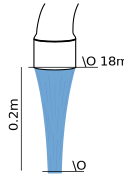
\includegraphics{fig/behoudsvergelijkingen/waterkraan}

\end{toepassing}
\begin{antwoord}{\ref{waterkraan}}
	$d = 5\unit{mm}$
\end{antwoord}
%%%%%%%%%%%%%%%%%%%%%%%%%%%%%%%%%%%%%%%%%%%%%%%%%%%%%%%%%%%%%%%%%%%%%%%%%%%%%%%%%%%%%%%%%
\begin{toepassing}[*]
	\label{hevel}
Een hevel wordt gebruikt om water uit een tank te halen, aan het uiteinde van de hevel heerst de atmosfeerdruk. De hoogtes zijn zoals aangegeven op onderstaande figuur, de buis heeft een constante diameter. Veronderstel dat het water zich niet viskeus gedraagt.
		
Bepaal de gemiddelde snelheid en de druk op het hoogste punt in de hevel.
	\centering
	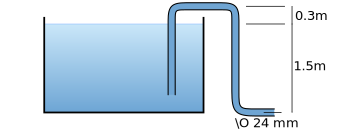
\includegraphics{fig/behoudsvergelijkingen/hevel}

\end{toepassing}
\begin{antwoord}{\ref{hevel}}
	$v = 5.42\unit{m/s}$, $p = 84\unit{kPa}$
\end{antwoord}
%%%%%%%%%%%%%%%%%%%%%%%%%%%%%%%%%%%%%%%%%%%%%%%%%%%%%%%%%%%%%%%%%%%%%%%%%%%%%%%%%%%%%%%%%
\begin{toepassing}
	\label{drukhoogte}
Een leidingstelsel is opgebouwd zoals weergegeven in onderstaande figuur. Er zijn twee verticale meetbuizen aangebracht om de druk in de leidingen te kunnen meten. In de leidingen stroomt water dat als niet viskeus beschouwd mag worden.
		
Bepaal de hoogte van de vloeistof in de twee meetbuizen t.o.v. het vloeistof niveau in de tank.

	\centering
	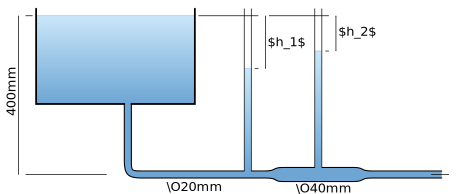
\includegraphics{fig/behoudsvergelijkingen/drukhoogte}
\end{toepassing}
\begin{antwoord}{\ref{drukhoogte}}
	$h_1 = 400\unit{mm}$, $h_2 = 25\unit{mm}$
\end{antwoord}
%%%%%%%%%%%%%%%%%%%%%%%%%%%%%%%%%%%%%%%%%%%%%%%%%%%%%%%%%%%%%%%%%%%%%%%%%%%%%%%%%%%%%%%%%
\begin{toepassing}
	\label{dynamische_druk}
Een een Pitot-buis en een manometer aangesloten op een leiding waarin lucht stroomt ($\rho=1.22\unit{kg/m^3}$). Beide buizen zijn aangesloten op een U-buis manometer waarin een olie met een dichtheid van 800\unit{kg/m^3} zit. De hoogteverschillen in de U-buizen zijn 0.2m en 0.6m zoals aangegeven op de figuur.

Bepaal de statische en de dynamische druk in de buis en de snelheid in de buis.

	\centering
	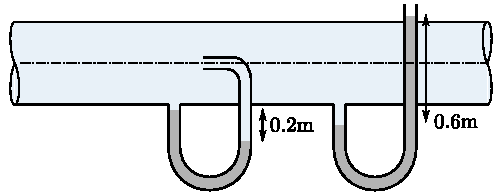
\includegraphics{fig/behoudsvergelijkingen/dynamische_druk}
\end{toepassing}
\begin{antwoord}{\ref{dynamische_druk}}
	$p_{\text{statisch}} = 4709\unit{Pa}$, $p_{\text{dynamisch}} = 1567\unit{Pa}$,\\ $v = 50.7\unit{m/s}$
\end{antwoord}
%%%%%%%%%%%%%%%%%%%%%%%%%%%%%%%%%%%%%%%%%%%%%%%%%%%%%%%%%%%%%%%%%%%%%%%%%%%%%%%%%%%%%%%%%
\begin{toepassing}
	\label{vernauwing}
Een vernauwing in een buis heeft afmetingen zoals afgebeeld op de onderstaande figuur. Door de buis stroomt olie met een dichtheid van 830\unit{kg/m^3}. De druk vlak voor de vernauwing is 2\unit{bar}. De stroming mag stationair en zonder wrijving verondersteld worden.
		
Bepaal de kracht uitgeoefend op de vernauwing ten gevolge van de stroming.

	\centering
	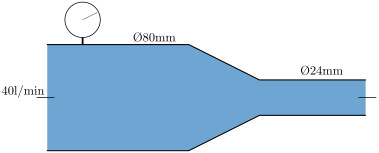
\includegraphics{fig/behoudsvergelijkingen/vernauwing}
\end{toepassing}
\begin{antwoord}{\ref{vernauwing}}
	$F = 919\unit{N}$
\end{antwoord}
%%%%%%%%%%%%%%%%%%%%%%%%%%%%%%%%%%%%%%%%%%%%%%%%%%%%%%%%%%%%%%%%%%%%%%%%%%%%%%%%%%%%%%%%%
\begin{toepassing}[*]
	\label{brandslang}
Het uitlaatstuk van een brandslang vormt een vernauwing van de slang diameter (50mm) tot de uitlaat (16mm). De stroming hierin mag zonder wrijving verondersteld worden.

Bepaal de kracht die uitgeoefend wordt op het uitlaatstuk indien er een debiet van 180 l/min water door de slang stroomt en we de zwaartekracht niet beschouwen.

	\centering
	%\includegraphics{fig/behoudsvergelijkingen/brandslang}
\end{toepassing}
\begin{antwoord}{\ref{brandslang}}
	$F_x = 176\unit{N}$
\end{antwoord}
%%%%%%%%%%%%%%%%%%%%%%%%%%%%%%%%%%%%%%%%%%%%%%%%%%%%%%%%%%%%%%%%%%%%%%%%%%%%%%%%%%%%%%%%%
\begin{toepassing}[*]
	\label{diffusiebocht}
Door een U-buis in een horizontaal vlak, met verlopende doorsnede, stroomt water met een intredesnelheid van 4m/s. De oppervlaktes van de doorsneden bij in en uittrede zijn gegeven in de figuur. De druk aan de intrede wordt gemeten en is 150\unit{kPa}.
		
Bepaal de grootte en de richting van de reactiekracht van de buis op het water.

	\centering
	
\includegraphics{fig/behoudsvergelijkingen/diffusiebocht}
\end{toepassing}
\begin{antwoord}{\ref{diffusiebocht}}
	$F = 97.2\unit{kN}$
\end{antwoord}
	
\section*{Antwoorden}
	\begin{multicols}{2}
		\includecollection{antwoorden}
	\end{multicols}